\section{介绍}

\begin{frame}{先声夺人}
  \centering
  \scalebox{5}{\textipa{/"leItEk/}}
\end{frame}

\begin{frame}{\LaTeX{} 是什么?\mbox{}——\mbox{}你为什么学}
\pause
\begin{itemize}
  \item<+-> Word 替代品?

    \begin{itemize}
      \item 「我受够了,我以后什么都要用 \LaTeX{} 写」
    \end{itemize}

  \item<+-> 写论文神器?

    \begin{itemize}
      \item 「我就是为大 paper 而生的,当然必须学 \LaTeX{} 啦」
    \end{itemize}

  \item<+-> 打公式方便?

    \begin{itemize}
      \item 「复杂公式输入哪家强,当然首选 \LaTeX{} 帮忙」
    \end{itemize}
\end{itemize}
\end{frame}


\begin{frame}[fragile]
\frametitle{\LaTeX{} 是什么?\mbox{}——\mbox{}What you \emph{think} is what you get!}
\begin{columns}
\begin{column}{0.48\textwidth}
  \centering
  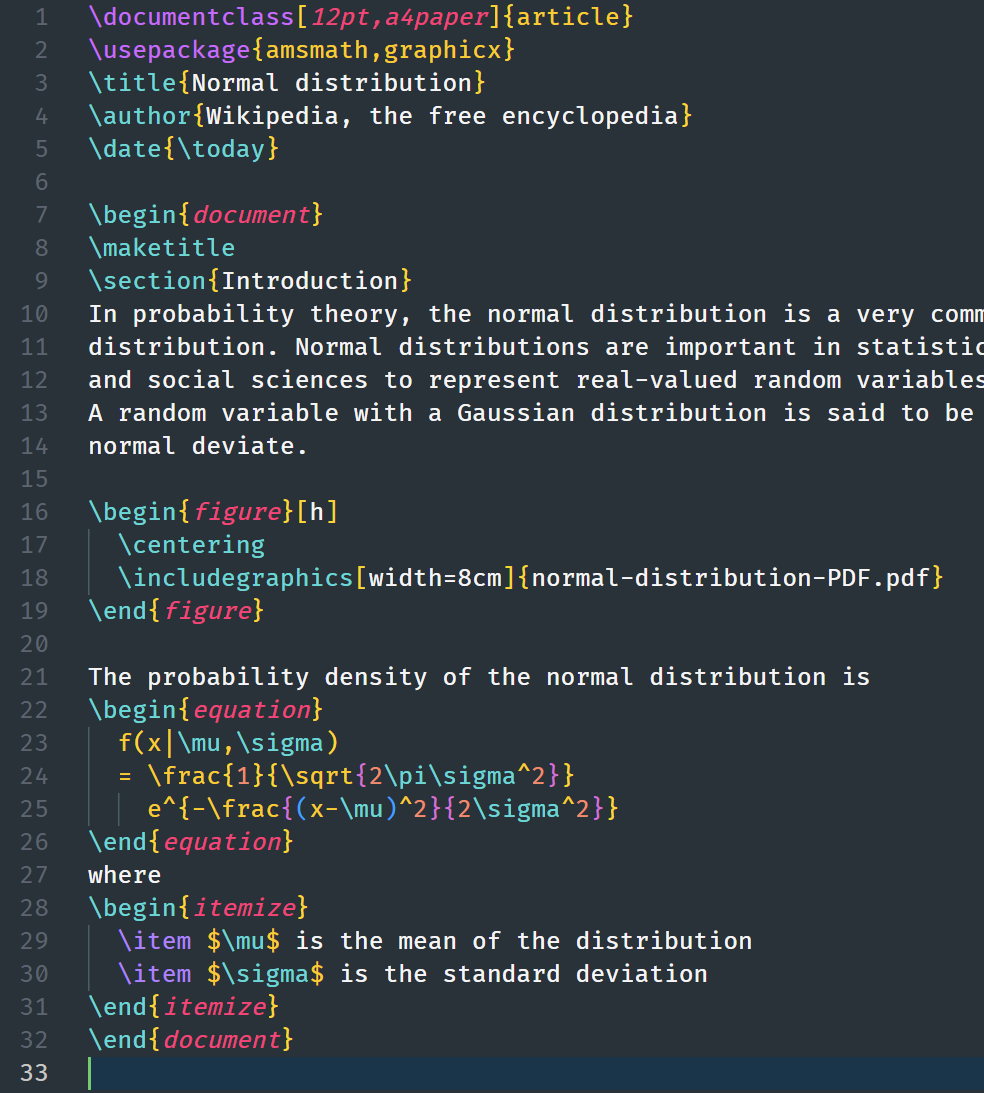
\includegraphics[width=0.75\textwidth]{images/code.png}
\end{column}
\begin{column}{0.48\textwidth}
  \begin{figure}
    \centering
    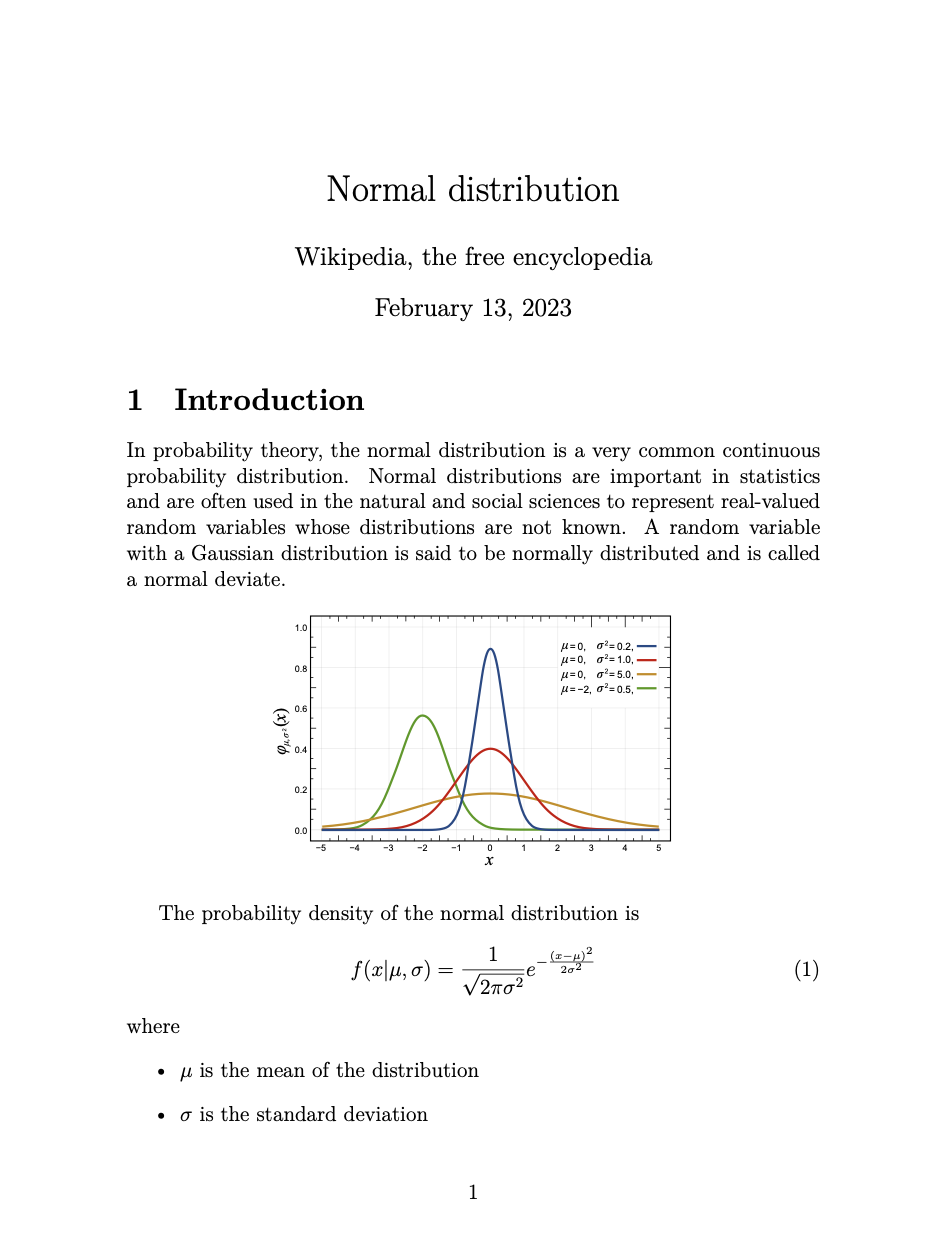
\includegraphics[width=0.75\textwidth]{images/normal-dist.png}
  \end{figure}
\end{column}
\end{columns}
\end{frame}

\begin{frame}{基本原则}
  \begin{itemize}
    \item<+-> 排版 vs 文字处理

      \begin{itemize}
        \item 《别把 \LaTeX{} 当 Word 用》
        \item {\scriptsize 在固定版面内,摆置各种不同类型的资料,以最合适的方法呈现 \href{https://zh.wikipedia.org/wiki/排版}{\faWikipediaW}}
      \end{itemize}

    \item<+-> 遵循业界规范
    \item<+-> 追求良好的阅读体验 (readability)
    \item<+-> 内容与格式分离
    \item<+-> \alert{内容永远比格式重要!}
  \end{itemize}
\end{frame}

\subsection{\TeX 排版系统历史}

\begin{frame}[fragile]{\TeX 与 \LaTeX{} 的起源}
  \begin{columns}[T]
    \column{.7\textwidth}
    \begin{itemize}
      \item \TeX: $\tau\varepsilon\chi$ (\textipa{/'tEx/},
        \textipa{/'tEk/})
        \begin{itemize}
          \item 生成精美图书的排版系统
          \item 最初由 高德纳\footnote{1974年图灵奖得主,《计算机程序设计艺术》(The Art of Computer Programming)作者。} (Donald E.~Knuth) 于 1978 年开发  
          \item 最新版本为 \TeX\ 3.14159265
          \item 漂亮、美观、稳定、通用
          \item 尤其擅长数学公式排版
        \end{itemize}

        \vspace{2em}
      \item \LaTeX{}(\textipa{/'la:tEx/}, \textipa{/'leItEk/})
        \begin{itemize}
          \item Leslie Lamport\footnote{2013年图灵奖得主,对于分布式及并形系统的理论与实践具有基础性贡献。} 开发的一种 \TeX 格式
          \item 在 \TeX 的基础上提供宏包, 降低使用门槛
          \item 极其丰富的宏包,提供扩展功能
          \item 广泛用于学术界,期刊会议论文模板
        \end{itemize}
    \end{itemize}
    \column{.2\textwidth}
    \vspace*{-5mm}
    \hspace{-10mm} 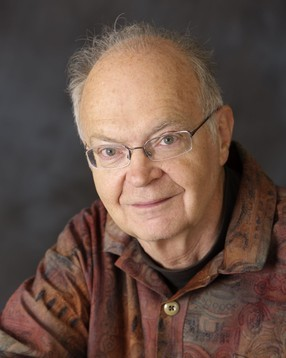
\includegraphics[width=\textwidth]{images/Knuth.jpg}

    % \vspace*{5mm}
    \hspace{-10mm} 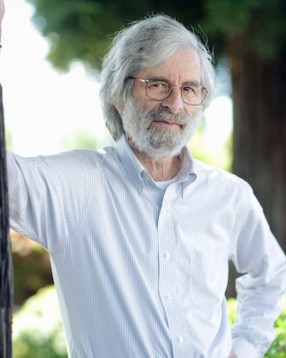
\includegraphics[width=\textwidth]{images/Lamport.jpg}

  \end{columns}
\end{frame}

\subsection{\LaTeX{} 利弊}

\begin{frame}[fragile]{\LaTeX{} 的好处与坏处}
    \textbf{好处}
    \begin{itemize}
        \item 数学公式排版优雅 \quad $\mathcal{F}(\xi)=\int_{-\infty}^{\infty} f(x)\mathrm{e}^{-\mathrm{j}2\pi \xi x}\,\mathrm{d}x$
        \item 内容与格式分离
        \item 随心所欲的宏定义与自定义命令 \rawcmd{\textbackslash newcommand},\rawcmd{\textbackslash def}
    \end{itemize}

    \pause

    \vspace{2em}
    \textbf{坏处}
    \begin{itemize}
        \item 得到易读的版本,需要编译
        \item 输入相对 Word 繁琐
        \item 非开箱即用。有时自行解决编辑器、宏包,甚至是编译错误。
    \end{itemize}

\end{frame}
